\begin{figure}[h!]
    \centering
    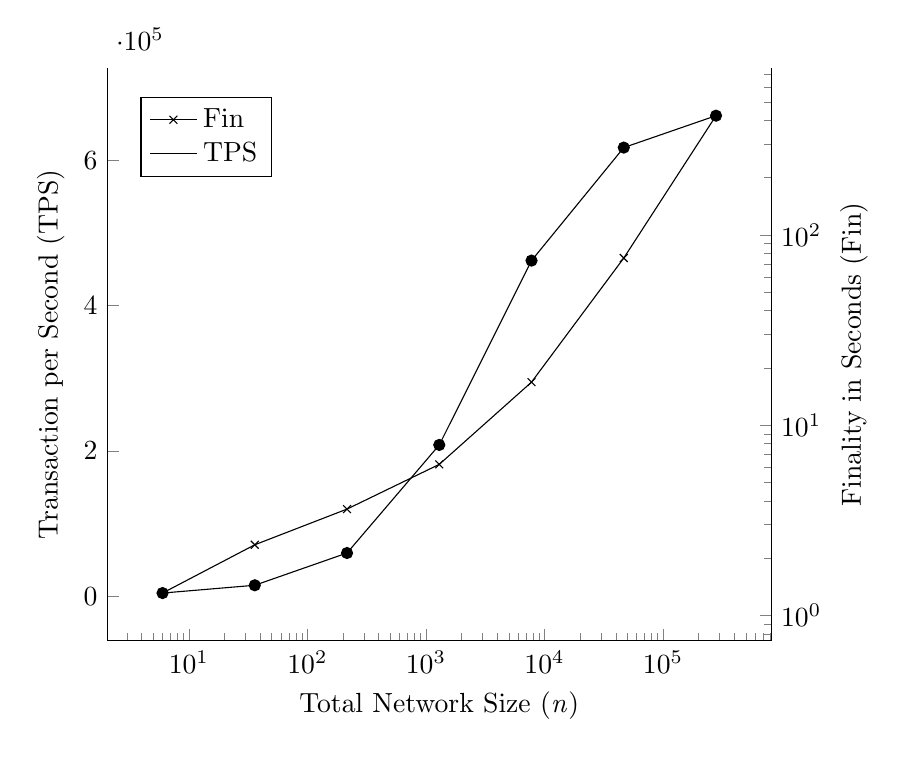
\begin{tikzpicture}
      \pgfplotsset{
          scale only axis,
      }
    
      \begin{axis}[
        xmode=log,
        axis y line*=left,
        axis x line*=bottom,
        xlabel = Total Network Size (\textit{n}),
        ylabel= Transaction per Second (TPS),   
        scaled y ticks=true
      ]
        \addplot[mark=*]
          coordinates{
            (6,4584.13)	
            (36,15298.09)	
            (216,59673.05)	
            (1296, 208362.67)	
            (7776,461963.52)	
            (46656,617451.49)	
            (279936,661354.75)
            % more points
          }; \label{plot_1}
    						
        \end{axis}
    
        \begin{axis}[
          xmode=log,
          ymode=log,
          axis y line*=right,
          axis x line*=bottom,
          axis x line=none,
          ylabel=Finality in Seconds (Fin),
          legend style={at={(0.05,0.95)}, anchor=north west, legend cell align=left},
        ]
    
        \addplot[mark=x]
          coordinates{
            (6,1.31)	
            (36,2.35)	
            (216,3.62)	
            (1296, 6.22)	
            (7776,16.83)	
            (46656,75.56)	
            (279936,423.28)			
            % more points
          }; \label{plot_2}
        \addlegendimage{/pgfplots/refstyle=plot_1}\addlegendentry{Fin}
        \addlegendimage{/pgfplots/refstyle=plot_2}\addlegendentry{TPS}
        \end{axis}
    \end{tikzpicture}
    \caption{The network throughput and finality as the number of network members increases, assuming the network is under maximum possible load.}
    \label{fig:proj_large}
\end{figure}